\documentclass[t]{beamer}
\input{\jobname_header}
\input{\jobname_beameranpassungen}

\NewDocumentCommand{\altTeX}{}{%
  \textsf{alt}\TeX\xspace
}

\begin{document}

\begin{frame}{Worum geht es?}
• Einfacherers Arbeiten mit \TeX\ durch:
• Maschinen: Neuentwicklungen der letzten Jahre, Nutzen für den normalen Anwender
• Formate: \LaTeX3-Kernel und Paket, die darauf basieren
• Tastaturen: Neo-Tastaturlayout
\•
\end{frame}

\section{Maschinen}
\begin{frame}{Maschinen}
• kurzer Überblick über die Entwicklung von \TeX78 bis lua\TeX\\
(aktuelle Version unter \url{http://github.com/alt/overview})
%%• im folgenden: nur \XeTeX\ und lua\TeX
\•
\end{frame}

\begin{frame}{Vorteile neuer Maschinen – im Alltag}
\begin{block}{Vollständige utf8-Unterstützung}
⇒ nie mehr Probleme beim Austausch von Dokumenten, nie wieder kaputte Umlaute, keine umständliche Eingabe von speziellen Zeichen anderer Sprachen, beliebig viele Sonderzeichen,\\
ganz zu schweigen von asiatischem Satz …
\end{block}

\begin{block}{moderne Schrifttechnologien (ttf, otf, aat)}
Keine speziellen Dateien zum Schrifteinbinden benötigt, Portabilität von Schriften anderer Anwendungen\\
⇒ modernste, neuste Schriften sind in vollem Funktionsumfang leicht verwendbar
\end{block}
\end{frame}

\begin{frame}{Nachteile neuer Maschinen}
\begin{block}{}
• etwas Neues muss gelernt werden
• weniger stabil (bugs/neue Features)
• nicht rückwärtskompatibel
• auf veralteten Systemen nicht verfügbar
• Wermutstropfen bei \XeTeX: Mikrotypographie nicht wie bei pdf\TeX\ möglich
• Verwirrung und Unklarheiten durch neue Vielfalt („Welche Maschine, welches Format, welche Distribution nutzt du?“)
\•
\end{block}
\end{frame}

\section{Formate}
\begin{frame}{Formate}
• fast niemand verwendet INITEX als Programm, fast immer wird ein Format verwendet:
• plain\TeX: Do It Yourself!
• \LaTeX: A Document Preparation System
• Con\TeX t: super-duper cow power – kann alles außer Dokumentation\pause
• alle Formate können an Maschinen angepasst werden, um bestimmte Features leicht zugänglich zu machen: pdf\LaTeX, \XeLaTeX, lua\LaTeX, Con\TeX t Mk II bzw. IV, plain lua\TeX\ etc.
\•
\end{frame}

\begin{frame}{The neverending story: \LaTeX3}   %% hat 448 Seiten und auch ein Ende …
• \LaTeXe: eigentlich als Zwischenversion zu \LaTeX3 geplant, inzwischen eingefroren und meistverwendetes \TeX-Format
• keine Weiterentwicklung im Kernel, keine Korrektur von Designfehlern
• \LaTeX3 als lange währendes, unbekanntes Mysterium …
• einige Pakete bauen bereits auf \LaTeX3-Code auf
• z.\,B. |siunitx|, |fontspec|
• inzwischen ist \LaTeX3 sogar bei lua\TeX\ angekommen …
\•
\end{frame}

\begin{frame}{Con\TeX t}
• baut in der neusten Verison voll auf lua\TeX\ auf
• kann alles außer Dokumentation
• wer mag, darf nun was dazu sagen …
\•
\end{frame}

\begin{frame}{Designmerkmale von \LaTeX3 (Auswahl)}
• Versuch einer „gesunden“ (sane) Programmierebene, die von \TeX\ abstrahiert
• gute, übersichtliche Namensgebung von internen Makros (großes Problem von \LaTeXe)
• sinnvolle Strukturierung etc. etc. etc.
\•
\end{frame}

\begin{frame}[fragile]{Designmerkmale von \LaTeX3 (Auswahl)}
• anderes Catcode-Regime: |\ExplSyntaxOn/Off|\\%
 (vgl. |\makeatletter \makeatother|
• Leerzeichen werden ignoriert (|~| wenn nötig)
• Namen: Das |@| als Trennstelle in Namen wird vom |_| übernommen
• Interne Namen enden mit einem |:|\pause
• Nach dem |:| werden erwartete Argumente dargestellt
• |\cs_new:Npn|\\%
|Modulname_Zwischenname_Name : Argumente|
\•
\end{frame}

\begin{frame}[fragile]{Argumente}
• |N|: „normal“es Token
• |n|: „normal“, gruppiert
• |e|: wird expandiert
• |x|: wird voll expandiert
• |c|: baute eine Kontrollsequenz: |\cs_new:cpn{name} = \cs_new:Npn\name|
• |p|: \TeX-Parametersequenz (|#1 xyz #2|)
• |T|: true-Zweig für |\if|-Abfragen
• |F|: false-Zweig für |\if|-Abfragen (T, F oder TF möglich!)
• |w|: „wired“ – alles andere (z.\,B. low level-|\if|-Konstrukte)
\•
\end{frame}

\begin{frame}{Vorteile der Namensgebung}
• Konsistente Einteilung in Module möglich
• Quellcode wesentlich besser lesbar (Wird eine Variable gesetzt? Ein Zähler? Eine Konstante verwendet? …)
• Anzahl der nötigen Argumente direkt sichtbar
• Ändern von Expansion/Auswertung etc. eines Argumentes durch Ändern eines Buchstabens im Argument
\•
\end{frame}

\begin{frame}[fragile]{Beispiel für sinnvolle \LaTeX3-Konstrukte}
• angenommen: Der Nutzer kann einen Namen |\name| vorgeben. Aus diesem Namen werden die Befehle |name1|, |name2| und |name-<name1>| gebaut. (|hallo| ⇒ |hallo1|, |hallo2|, |hallo-Inhalt 1|)
\•
\begin{block}{\TeX, meist in \LaTeX\ verwendet:}
\begin{verbatim}
\expandafter\def\csname \name1\endcsname{Inhalt 1}
\expandafter\def\csname \name2\endcsname{Inhalt 2}
\expandafter\def\csname \name-\csname\name \endcsname\endcsname{Inhalt von name-<name>}
\end{verbatim}
\end{block}

\begin{block}{\LaTeX3}
\begin{verbatim}
\ExplSyntaxOn
\cs_new:cpn{\name1}{Inhalt 1}
\cs_new:cpn{\name1}{Inhalt 2}
\cs_new:cpn{\name1-\cs:w \name \cs_end:}{Inhalt 1}
\ExplSyntaxOff
\end{verbatim}
\end{block}
\end{frame}

\begin{frame}[fragile]{\LaTeXe-Versionen}
\LaTeXe\ bietet u.\,a. |\@nameuse| und |\@namedef| – aber recht selten genutzt (mir bis 4 Tage vor diesem Vortrag nicht bekannt, dass es Verwendung findet)
\end{frame}

\begin{frame}[fragile]{Beispiel für das Arbeiten mit \LaTeX3}{levelscheme.dtx}
• bestes Beispiel für Arbeit mit \LaTeX3: \LaTeX3-Kernel (|texdoc source3|)
• für alles andere: |expl3| unter \LaTeXe
• |expl3| bietet grundlegendes Programmierinterface
• bietet viele Lösungen, für die \LaTeXe\ nur sehr umständliche Konstrukte hatte
• Pakete, die nicht zum eigentlichen Kernel gehören, bieten high-level Interface für den normalen Nutzer
• z.\,B. |xparse| 
\•
\end{frame}

\begin{frame}[fragile]{xparse}{Definieren von Dokumentbefehlen}
• bietet ein sehr effizientes Interface zum Definieren von Dokumentbefehlen (für den Endnutzer gedachte Befehle)
• |\(Declare/New/Renew/Provide)| – |Document| – |(Command/Environment)|
• für Paketautoren und normale Nutzer
• erfordert keine \LaTeX3-Syntax (nur intern damit programmiert)
• Argumente werden einzeln aufgezählt
• verschiedene Arten von Argumenten beliebig mischbar
\•
\end{frame}

\begin{frame}[fragile]{xparse}{Anwendung}
•[L2] |\newcommand\mycommand[2]{<Definition>}|
•[L3] |\NewDocumentCommand\mycommand{mm}{<Definition>}|\\%
~\pause
•[L2] |\newcommand\mycommand[opt][2]{<Definition>}|
•[L3] |\NewDocumentCommand\mycommand{O{opt}m}{<Definition>}|\\%
~\pause
•[L2] ???
•[L3] |\NewDocumentCommand\mycommand{sO{opt}mt{A}O{2nd opt}mm}{<...>}|\\%
Aufruf: |\mycommand*[Option1]{Argument} A [Option2] {Argument2}{Argument3}|
\•
\end{frame}

\begin{frame}[fragile]{xparse}{Argumenttypen – Auswahl}
•[m] mandatorisch, Gruppe oder einzelnes Token
•[o] optional, wird zu |-NoValue-| wenn nicht gegeben
•[O\{\}] optional, wird zum Argument, wenn nicht gegeben
•[t\{\}] es wird geprüft, ob das in Klammern gegebene Token vorkommt (boolscher Test)
•[s] testet, ob ein Stern vorkommt (= |t{*}|)
•[u\{\}] liest bis zum angegebenen Token
•[d12] optionales Argument, das durch die Token |1| und |2| begrenzt ist, z.\,B. |t<>|
•[] l, D, g, G
\•
\end{frame}

\begin{frame}{Anwendungsbeispiel}
\begin{block}{levelscheme}
Ein Paket, das das einfache Zeichnen von atomaren Levelschemata ermöglicht. Intern in |expl3| geschrieben, Nutzerbefehle mittels |xparse| geschrieben.
\end{block}
\end{frame}

\begin{frame}[fragile]{fontspec v2}
• |fontspec| hat \XeTeX\ für \LaTeX-Nutzer erst richtig interessant gemacht
• sehr einfaches und mächtiges Interface für sämtliche Schriftfeatures\pause
• in Version 2: auch für lua\TeX
• gleiche Syntax für den Nutzer, aber (fast) alle features von lua\TeX\ verfügbar
• Code zum Schriftladen von Con\TeX t kopiert und verwendet
• größtenteils in \LaTeX3-Syntax geschrieben
\•
\end{frame}

\begin{frame}[fragile]{fontspec v2}
• |\setmain/mono/sansfont{Schriftname}|
• unter \XeTeX: Schriftname muss der sein, unter dem das Betriebssystem die Schrift kennt!
•[⇒] abhängig vom System!
• unter lua\TeX: Schriftdatenbank, alle Namen einer Schrift verfügbar (Schriftname, Systemname, Name für Menschen, Dateiname etc.)
• falls vorhanden, werden zugehörige Schnitte bei Bedarf eingebunden
•[⇒] |\fontspec{Linux Libertine} \textit{test}| lädt die Libertine in kursivem Schnitt
\•
\end{frame}

\section{Neo – ein Tastaturlayout}
\begin{frame}{Was haben \TeX\ und Tastaturbelegungen gemeinsam?}
•<+> Sie sind alt!
• die am weitesten verbreitete Belegung |qwerty/z| kam 1868 auf
• \TeX\ kam 1978 in der ersten Version raus
• seitdem hat sich bei \TeX\ einiges getan – bei Tastaturen nicht
• da die Tastatur das wichtigste Hilfsmittel ist – betrachten wir die Entwicklung der beiden Ts und schauen, wie sie voneinander profitieren können
\•
\end{frame}

\begin{frame}{Tastaturbelegungen – ganz kurz}
• Tastatur\emph{belegung} – es geht nicht um ergonomische Hardware!
• Anordnung der Tasten, Zeichenauswahl etc. noch von uralten Schreibmaschinen beibehalten
• nur wenige, kleine Änderungen (|y| und |z| im Deutschen getauscht, Umlaute)
• kaum Rücksichtnahme auf Erogonomie
• Belegung durch mechanische Bedingungen gegeben
\•
\end{frame}

\begin{frame}[fragile]{Neo – ein Tastaturlayout}
• Hauptziel: ergonomische Tastaturbelegung
• schnelles Schreiben (auch mit unergonomischen Belegungen möglich)
• angenehmes Schreiben (geringe Laufwege für Finger entlasten Gelenke)\pause
• Nebenziel/Nebeneffekt: Große Vielzahl an Sonderzeichen leicht erreichbar
• Ergonomie: statt Rumklicken oder Zahleneingabe: Tastenkombination\\%
|Ξ√Λℂ⊂∫∀∃∪∩ΠℵΨΓΦℚ⇔↦⇒ΣΔ … |
\•
\end{frame}

\begin{frame}[fragile]{Neo – ein Tastaturlayout mit vielen Sonderzeichen}
• erreichbar über zusätzliche Modifier
• maximal zwei Modifier plus Taste
• für noch mehr Sonderzeichen: Compose-Taste\\%
(unter Linux und Solaris bekannt, jetzt auch für Windows, und stark erweitert)
\•
\end{frame}

\begin{frame}{Neo – Ebenen 1 und 2:}
\input{ebene12}
\end{frame}

\begin{frame}{Neo – Ebene 3:}
\input{ebene3}
\end{frame} 

\begin{frame}{Neo – Ebene 6:}
\input{ebene6}
\end{frame} 

\section{Experimente mit \altTeX}
\begin{frame}{Was ist \altTeX?}
• experimentelles Paket zum „alternativen \TeX en“
• Ansätze, die häufige Arbeiten einfacher machen
• stark auf Neo aufbauend (Verwendung vieler unicode-Zeichen)
• 
\•
\end{frame}

\begin{frame}[fragile]{Itemize}
• Aufzählung im normalen Text:
\begin{verbatim}
\begin{itemize}
\item erster Punkt
\item zweiter Punkt
\end{itemize}
\end{verbatim}
• recht viel Schreibarbeit
• ein guter Editor kann sehr viel Arbeit abnehmen
• aber Code schlecht lesbar
\•
\end{frame}

\begin{frame}[fragile]
• Idee: Nehme ein freies Unicodezeichen (z.\,B. |•|)
• weise dem Zeichen eine Bedeutung zu, die seinem Aussehen entspricht (z.\,B. Aufzählungspunkt)
• implementiere so, dass kein weiterer Code nötig ist (Umgebungen etc.)
\•
\end{frame}

\begin{frame}[fragile]{Beispiel: itemize}
• Ziel: der Code soll genau das tun, wonach er aussieht:
\begin{verbatim}
normaler Text

• erster Punkt
• zweiter Punkt

weiter im Text
\end{verbatim}
•[⇒] Äufzahlung ohne weitere \TeX-Befehle
\•
\end{frame}

\begin{frame}[fragile]{Beispiel: itemize}
• erster Ansatz: |•| aktiv machen
\begin{verbatim}
\catcode\`• = \active
\end{verbatim}
\pause
• Bedeutung zuweisen:
\begin{verbatim}
\let • \item
\end{verbatim}
• Bereits Verbesserung im Lesefluss:
\begin{verbatim}
\begin{itemize}
• erster Punkt
• zweiter Punkt
\end{itemize}
\end{verbatim}
\•
\end{frame}

\begin{frame}[fragile]{Beispiel: itemize}
• weiterhin: Umgebung |\begin{verbatim}| einsparen!
• dazu: bei jedem Auftreten von |•| prüfen, ob man bereits in der Aufzählung ist:\pause
\•
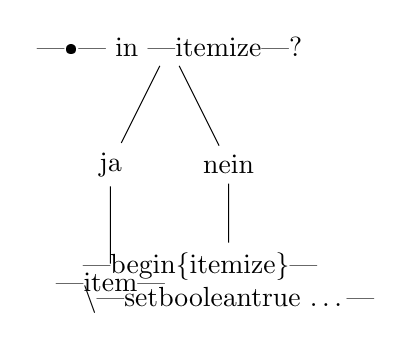
\begin{tikzpicture}
\node {|•| in |itemize|?}
    child {node {ja}
      child {node {|item|}}}
    child {node {nein}
      child {node {\vbox{\hbox{|begin\{itemize\}|}\hbox{\textbackslash|setbooleantrue …|}}}}}
;
\end{tikzpicture}
\end{frame}

\begin{frame}[fragile]{Beispiel: itemize}
• schließlich: |\end{verbatim}| einsparen
• Problem: kein Zeichen zum Beenden verwendet!
•[⇒] wann weiß \TeX, dass die Umgebung beendet werden soll?\pause
• Ansatz: Eindeutige Sequenz beendet die Umgebung: Doppeltes Zeilenende (= Leerzeile)
•[⇒] definiere Zeilenende als Makro, das überprüft, ob es ein- oder zweimal aufgetreten ist
• falls zweimal: beende Umgebung und setze Zeilenende auf normale Bedeutung zurück
\•
\end{frame}

\begin{frame}[fragile]{Beispiel: itemize}
\begin{verbatim}
\cs_new:Npn\newitemi{%
  \if_meaning:w\insideitemizei\inside%
    \cs_set_eq:NN\altlastitem1%
    \exp_after:wN\item%
  \else:%
    \begin{itemize}%
    \cs_set_eq:NN\insideitemizei\inside%
    \cs_set_eq:NN\altlastitem1%
    \makeenteractive%
    \exp_after:wN\item%
  \fi:
}
\end{verbatim}
\end{frame}

\begin{frame}[fragile]{\altTeX für den Mathesatz}{Unicodezeichen im Mathesatz}
• Schreiben von Unicodezeichen als Mathesatz: Paket |unicode-math| von Will Robertson\pause
• Ermöglicht direkte Eingabe aller mathematischen Zeichen unter Verwendung von OpenType-Matheschriften
• |∫₀⁸ x² = 170 ⅔| $\int _0^8 x^2 = 170 \frac23$
\•
\end{frame}

\begin{frame}[fragile]{\altTeX für den Mathesatz}{Hoch- und Tiefstellen}
• Schreiben vieler hoch- und tiefgestellter Zahlen (z.\,B. Tensorrechnung) ist sehr lästig
•[⇒] Ziel: Einsparen von Gruppierungen!
• Ansatz: Definiere |_| und |^| als Makros, die ihr Argument bis zum nächsten Leerzeichen suchen, falls keine Klammer geöffnet wird
• Alles zwischen |_|,|^| und einem Leerzeichen wird als Argument hoch- bzw. tiefgestellt
• erspart immens viel lästige Schreibarbeit
• nur für kurze Argumente geeignet, da aber am nützlichsten
• bei langen Argumenten: wie üblich gruppieren
\•
\end{frame}

\begin{frame}[fragile]{\altTeX für den Mathesatz}{Klammersetzen}
• Klammern müssen fast immer mit |\left| und |\right| gesetzt werden:
\•
\begin{LTXexample}
\[(\frac 12) \left(\frac 12 \right)\]
\end{LTXexample}
•[⇒] Ziel: Klammern werden immer angepasst
• Ansatz: Sichere Bedeutung von |()| in Makros |\openbrace \closebrace|
• mache |()| aktiv
• definiere |()| als |\left\openbrace| bzw. |\right\openbrace|\pause
• Problem: Jegliche andere Verwendung von Klammern (im Text, bei |picture|-Umgebung u.\,ä.) funktioniert nicht mehr!
• Abfangen durch geschicktere Definition, Überprüfen des Mathemodus etc.
\•
\end{frame}

\begin{frame}[fragile]{\altTeX für den Mathesatz}{Matrizen}
• Eingabe von Matrizen ist recht aufwändig und unübersichtlich:
\•
\begin{LTXexample}
$\begin{bmatrix} a & b \\ c & d \end{bmatrix}$
\end{LTXexample}
• Unicode verfügbt über Klammern, die zum Einschließen von Matrizen geeignet sind
• mit Neo leicht zu erzeugen über Compose-Funktion:
\•
\begin{verbatim}
♫ x <Klammertyp> <Anzahl Spalten>
♫ x ( 3
⎛⎞
⎜⎟
⎝⎠
\end{verbatim}
\end{frame}


\begin{frame}[fragile]{\altTeX für den Mathesatz}{Matrizen}
• Idee: wieder aktive Zeichen
• erstes Klammerzeichen (links oben) beginnt die Matrix, setzt andere Zeichen auf die entsprechenden Makros
• alle rechten Klammerzeichen sorgen für einen Zeilenumbruch in der Matrix
• zur Sicherheit: rechte Klammerzeichen ignorieren das nächste Zeichen ⇒ verhindert Doppelausführung, falls rechte und linke Begrenzungen identische Zeichen sind
• das letzte rechte Zeichen beendet die Matrix
\•
\end{frame}

\begin{frame}[fragile]{\altTeX für den Mathesatz}{Matrizen}
• weitere mögliche Verbesserung: Definiere den Tabulator als Zellentrennzeichen |&| ⇒ keine Steuerzeichen stören die Matrix, sie passt hervorragend ins Dokument, an Tabulatoren ausgerichtet\pause
• Nachteil: Schreiben mitten in der Zeile ist nicht möglich, da \TeX\ zeilenweise einliest:
\•
\begin{verbatim}
a  = ⎛⎞
     ⎜⎟
     ⎝⎠ + b
\end{verbatim}
Außerdem keine Matrizen mit verschiedenen Klammern möglich ⇒ ließe sich aber implementieren, wenn die Eingabe möglich wäre.
\end{frame}

\begin{frame}{Quellen, Links, Verweise}
Quellcode für alt\TeX, \TeX-overview, |levelscheme| und diesem Vortrag:\\
\url{http://github.com/alt}\\
\LaTeX3 Quellen und Dokumentation: |texdoc source3| in einem aktuellen \TeX live und unter\\
\url{http://www.latex-project.org/latex3.html}\\
fontspec, unicode-math und alles andere von Will Robertson:\\
\url{http://github.com/wspr}\\
The official successor of \TeX:\\
\url{http://river-valley.tv/tug-2010/an-earthshaking-announcement}

\end{frame}


\end{document}

